\documentclass[12pt,twoside]{article}

\usepackage{paperlighter}

% Recommended, but optional, packages for figures and better typesetting:
\usepackage{microtype}
\usepackage{graphicx}
\usepackage{subfigure}
\usepackage{booktabs} % for professional tables

% Attempt to make hyperref and algorithmic work together better:
\newcommand{\theHalgorithm}{\arabic{algorithm}}


% For theorems and such
\usepackage{amsmath}
\usepackage{amssymb}
\usepackage{mathtools}
\usepackage{amsthm}

% if you use cleveref..
\usepackage[capitalize,noabbrev]{cleveref}


% Todonotes is useful during development; simply uncomment the next line
% and comment out the line below the next line to turn off comments
\usepackage[textsize=tiny]{todonotes}



\slimtitle{CNNs for the Prediction of ASD and Biomarker Identification}
\slimauthor{Tony Kabilan Okeke}

% ---------------------------------------------------------------------------------------
\begin{document}

% Article Information
\lightertitle{Convolutional Neural Networks for the Prediction of ASD and Biomarker Identification}
\lighterauthor{Tony Kabilan Okeke$^{\dagger}$}

% ----------------------------------- MAIN TEXT -----------------------------------------

\section{Introduction}

% Introduce the underlying biological questions asked by the authors (provide background)
Neuromodulation describes the process by which neuronal activity is regulated by exerting control over the physiological levels of various neurotransmitters. Neuromodulators are a special type of neurotransmitters which are released in a diffuse manner - not released at synapse alone, instead the entire neural tissue may be exposed to these molecules \cite{WhatNeuromodulation2009}. There are a variety of neuromodulators present in the brain, including Noradrenaline, Acetylcholine and Dopamine. These neuromodulators are known to elicit different effects in the brain. In the study titled "The Role of Neuromodulation in Cortical Plasticity: A Computational Perspective" by Pedrosa and Clopath specifically investigates two neuromodulatory effects  - 1) the gating of plasticity by altering the spike-time-dependent plasticity (STDP) learning window \cite{pedrosaRoleNeuromodulatorsCortical2017}, and 2) the upregulation of neuronal activity. The goal of this study was to investigate the potential effects of neuromodulators on receptive field plasticity. To accomplish this, they developed four hypothesized learning windows, each of which was represents the impact of different neuromodulators on the STDP learning curve. They then used a computational model to assess the consequences of these windows on receptive field plasticity. Finally, they compared the impact of upregulating the neuronal learning rate to the impact of upregulating neuronal activity assuming a standard antisymmetric STDP rule. \cite{pedrosaRoleNeuromodulatorsCortical2017}.

% Introduce the biological question you are asking (provide background – why is this question interesting?). Your question must be different from the research questions investigated in the paper.
The original study investigated the impact of neuromodulators on cortical plasticity, specifically by investigating the relationship between cortical plasticity, learning rate and neuronal activity. In their analysis, they focused on an antisymmetric STDP rule. In this paper, I will investigate how a symmetric STDP - which are known to facilitate the formation of a structure of neuronal assemblies in memory networks \cite{manzPurelySTDPbasedAssembly2023} -  rule alters the neuromodulatory influences on cortical plasticity as compared to the antisymmetric STDP rule. This investigation is particularly interesting since symmetric STDP rules have been associated with the stability and overlap of memory assemblies, which are necessary for the formation of strong associations between concepts encoded in the brain \cite{manzPurelySTDPbasedAssembly2023}.


\section{Methods}

\subsection{Original Paper}

%  Describe the mathematical model the authors used to ask their questions.
\textbf{Neuromodulatory States.} The researchers defined four distinct neuromodulatory states, each defined by a different learning rule for excitatory synapses. The first, referred to as the \textit{Depression-Potentiation} (DP) rule is the standard antisymmetric STDP rule, whereby a presynaptic spike preceding a postsynaptic action potential leads to potentiation of synaptic connections; this rule is observed in the visual cortex when both noradrenaline and acetylcholine are present \cite{seolNeuromodulatorsControlPolarity2007}. Second is the \textit{Potentiation-Potentiation} (PP) rule that a  symmetric STDP rule whereby all pairs of pre- and post-synaptic spikes cause potentiation; this rule is observed in the adult visual cortex when there is $\beta$-adrenergic receptor activation \cite{seolNeuromodulatorsControlPolarity2007}. Third is the \textit{Unchanged-Potentiation} (UP) rule whereby only the presynaptic spikes which are followed by postsynaptic action potentials trigger synaptic weight transitions that cause potentiation; it is observed in the lateral amygdala when there is dopaminergic action via D2 receptors \cite{pedrosaRoleNeuromodulatorsCortical2017}. Finally, the fourth rule is the \textit{Depression-Unchanged} (DU) rule whereby  synaptic weights are weakened each time a postsynaptic spike precedes presynaptic action potentials and remains unchanged; it is observed in the prefrontal cortex under nicotinergic modulation \cite{pedrosaRoleNeuromodulatorsCortical2017}.

\textbf{Effect of Neuromodulation on Cortical Plasticity.} The researchers developed a simple feedforward network which included a set of presynaptic input neurons projecting onto one postsynaptic neuron. The input neurons fire with time-varied firing rates following a Poisson distribution. The neurons were implemented as integrate-and-fire neurons with plastic excitatory synapses.  To evaluate the effect of different neuromodulatory states on cortical plasticity, the researchers simulated the feedforward network under each of the four neuromodulatory states described above. In practice this was accomplished by setting the pre- and post-synaptic amplitudes to different pre-determined values \cite{pedrosaRoleNeuromodulatorsCortical2017}.

\textbf{Modulation of Neuronal Activity vs Learning Rate.} In this case, the researchers developed a separate feedforward network with only one presynaptic and one postsynaptic neuron. The synaptic weights set according to the DP learning rule. The researchers goal was to compare the effects of upregulating neuronal activity and upregulating the learning rate. To assess the relationship between plasticity and learning rate, they calculated the ratio between synaptic weight change and actual synaptic weight and plotted that as a function of the learning rate. To assess the relationship between plasticity and neuronal activity, they calculated the ratio between the synaptic weight change and the actual synaptic weight and plotted that as a function of the presynaptic firing rate \cite{pedrosaRoleNeuromodulatorsCortical2017}. 

\subsection{My Work}

% Describe how the mathematical model has been altered by you to answer your specific question.
\textbf{Neuromodulatory Influences on Cortical Plasticity with Symmetric STDP.} To investigate this, I will utilize the same code and approach used to investigate the differences between modulating neuronal activity and modulating the learning rate. I will simulate the feedforward network with 10 presynaptic neurons and one postsynaptic. I will simply replace the parameters for the DP learning rule (antisymmetric STDP) with the parameters for the PP learning rule (symmetric STDP). I will then compare the results of the two simulations to determine the impact of the symmetric STDP rule on the neuromodulatory influences on cortical plasticity. 


\section{Results}

\subsection{Original Paper}

% Provide a summary of the authors’ results.
The researchers found that standard STDP rules with a depression component that was larger that the potentiation component lead to symmetry breaking of synaptic weights. This implies that some synaptic weights were strengthened while others were weakened. They also found that only the DP rule allowed for the emergence of receptive fields in the simple network model they employed. This suggests that by enhancing the action of neuromodulators like acetylcholine and noradrenaline in the visual cortex, one could facilitate the creation of receptive fields in the visual cortex \cite{pedrosaRoleNeuromodulatorsCortical2017}.

Additionally, the researchers also found that the potentiation-potentiation rule was more efficient for receptive field plasticity than other rules due to it having the largest amount of potentiation. This rule, PP is associated with the action of noradrenaline in the visual cortex, which indicates that noradrenaline could be a good candidate neuromodulator for facilitating receptive field plasticity in this region \cite{pedrosaRoleNeuromodulatorsCortical2017}.

Finally, the researchers found that modulating either the learning rate, or the neuronal activity lead to different alterations to synaptic weights. By upregulating the learning rate, they observed a sharpening of the receptive field. On the other hand, increasing presynaptic activity appeared to broaden the tuning. This seems to suggest that regulation of activity can lead to scenarios where weak weights learn faster than strong weights, indicating the potential for further broadening receptive fields.


\begin{figure}[ht]
    \vskip 0.2in
    \begin{center}
    \centerline{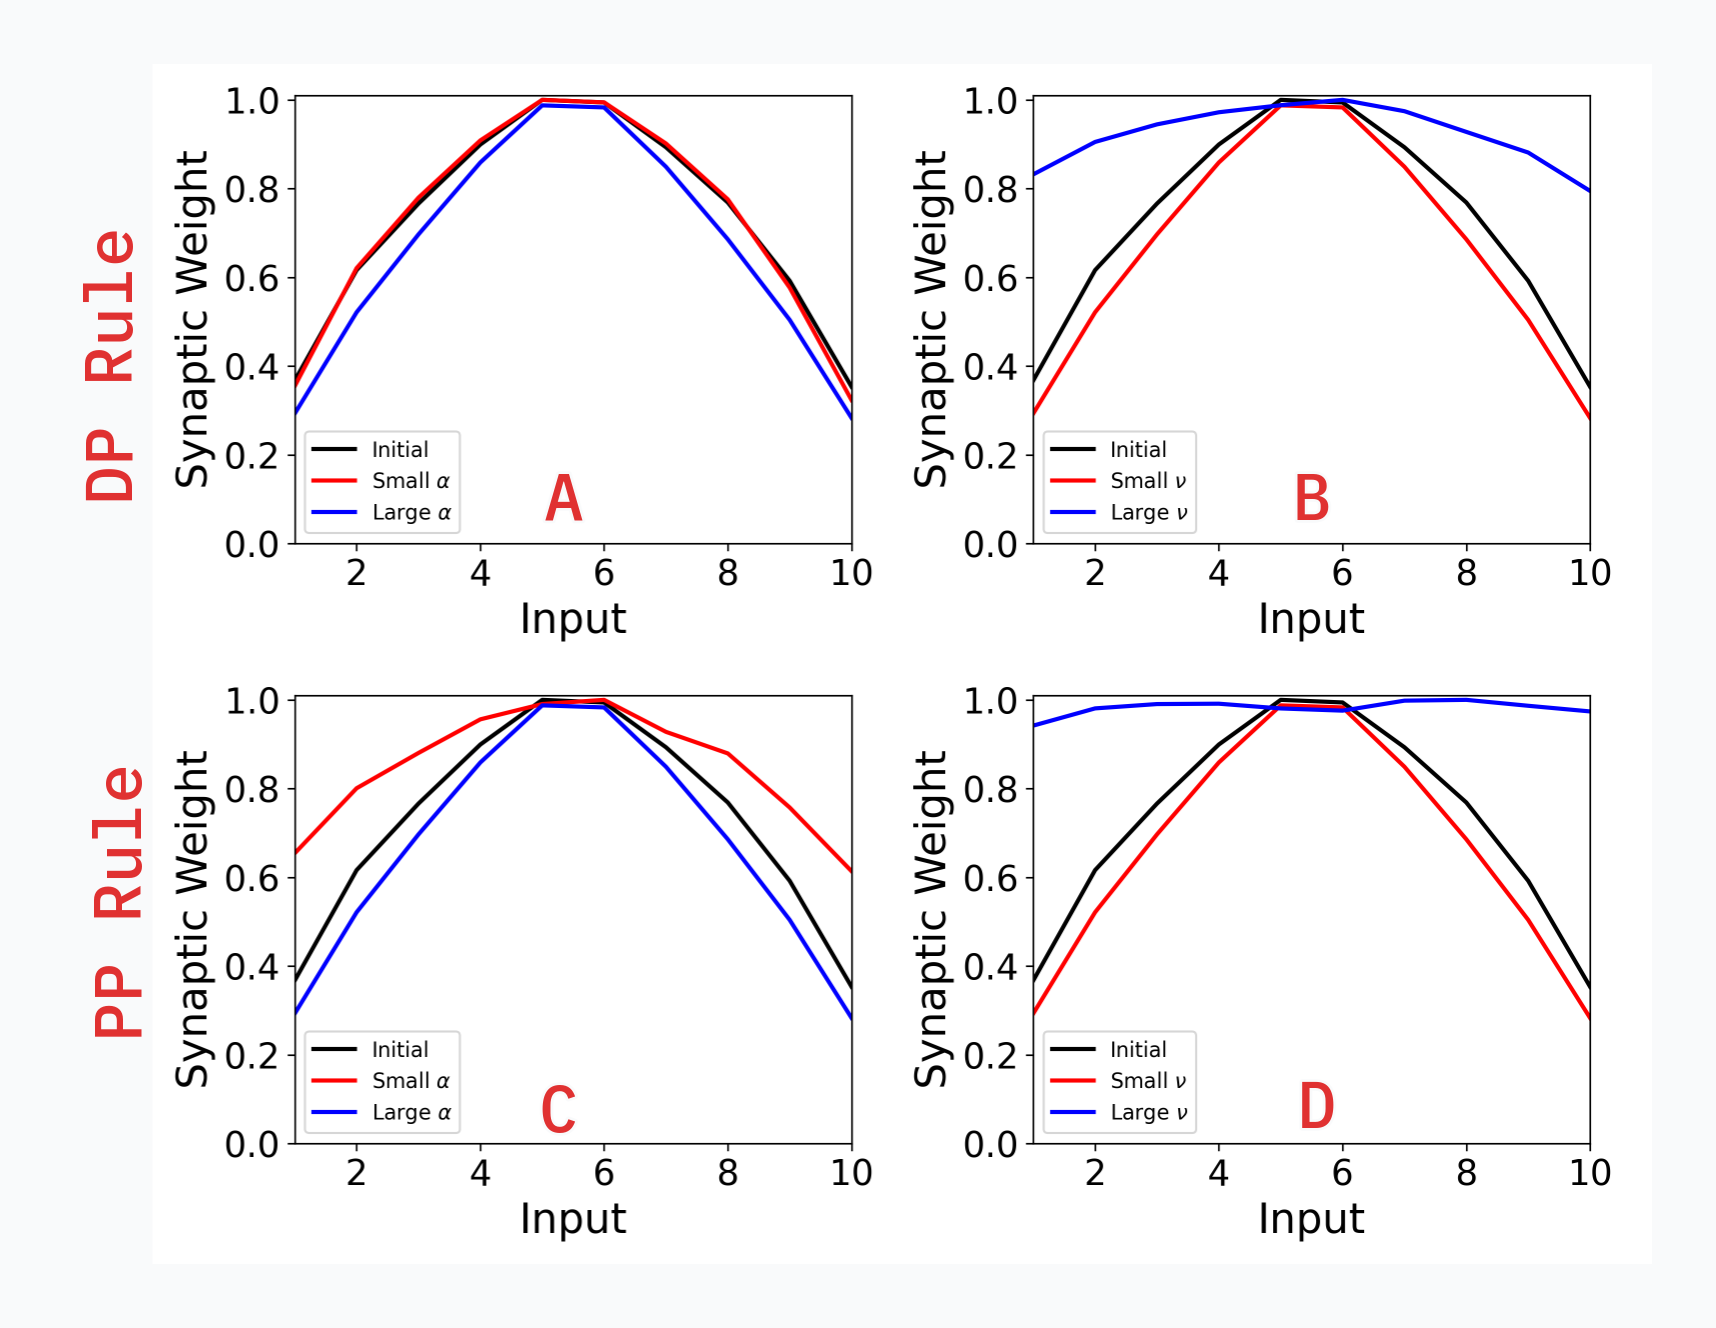
\includegraphics[width=4in]{figures/figure-1.png}}
    \caption{The impact of different STDP rules on the neuromodulatory influences on cortical plasticity. A) Synaptic weights for feedforward network using the DP STDP rule. The final synaptic weights were calculated for low presynaptic activity and two values for learning rate: 0.01, 0.02. The initial and final tuning curves were re-scaled by dividing all the tuning curves by their respective maximum weights. B) Synaptic weights for feedforward network using the DP STDP rule. The final synaptic weights were calculated for learning rate of 0.02 and 2 values of presynaptic activity: 1Hz and 10Hz. The initial and final receptive fields were scaled by dividing all the tuning curves by their respective maximum weights. C) Synaptic weights for feedforward network using the PP STDP rule. The final synaptic weights were calculated for low presynaptic activity and two values for learning rate: 0.01, 0.02. The initial and final tuning curves were re-scaled by dividing all the tuning curves by their respective maximum weights. D) Synaptic weights for feedforward network using the PP STDP rule. The final synaptic weights were calculated for learning rate of 0.02 and 2 values of presynaptic activity: 1Hz and 10Hz. The initial and final receptive fields were scaled by dividing all the tuning curves by their respective maximum weights.} 
    \label{figure-1}
    \end{center}
    \vskip -0.1in
    \end{figure}

\subsection{My Work}

% Describe the results you generated (make sure to include figures that clearly display your findings as related to your biological question)
As I investigated the impact that symmetric STDP would have on cortical plasticity, I utilized the codebase provided by the original authors as a starting point. I replicated the results they generated using the DP learning rule - although due to the computation time, I chose to limit my simulations to 2 trials instead of the original 20. I then replaced the parameters for the DP learning rule with parameters for PP learning rule. I then ran the simulation for 2 trials and plotted the results. The results of my simulations are shown in Figure \ref{figure-1}.

The results I generated diverged notably from those observed under the DP rule. The original study's results for the learning rate variation indicated a lot of overlap between the initial and small values, with a reduction in synaptic weight for the larger learning rate. However, for the PP rule, we see a more graded response with the smallest being the furthest out, then the initial, and finally the largest learning rate. For the presynaptic activity variation, the original study results exhibit higher weights for the larger presynaptic activity, decreasing as the presynaptic activity decreases. For the PP rule we generally see the same trend but with much higher synaptic weights on the large presynaptic activity end.


\section{Discussion}

% Evaluate whether the model has been applied appropriately and the model limitations.
The modifications made to the original codebase to produce these results were minimal, only changing a handful of paramenters to implement the symmetric STDP rule. This ensures that the model was used correctly and that the results are valid.  The replication of the results from the original study, albeit with a reduced number of trials, served as a good first step in establishing a baseline for comparison. The transition from antisymmetric DP to symmetric PP STDP rules was also straightforward, and the results were consistent with the findings of the original study.

However, the limitations of the model and the study design deserve careful examination. Constraining my analysis to 2 trails - a major deviation from the >= 20 trials conducted in the original study, could introduce variability that may not be representative of broader trends or may mask subtle effects that would have been evident with a larger sample size.

% Discuss the overall impact of the research paper as well as the overall impact of your modeling work. 
The original paper has contributed significantly to the field of neural engineering by provided a basic computational framework to explore the effects of neuromodulation on cortical plasticity. Their work utilizing different neuromodulatory states to investigate the impact of neuromodulation on cortical plasticity is particularly interesting since it provides a potential mechanism for the formation of receptive fields in different parts of the brain. My modeling work, which introduces the symmetric STDP rule into this existing framework, extends the impact of the original research by examining the potential for a more generalized model of synaptic potentiation, which could have implications for the design of neural network-based learning algorithms.


% ---------------------------------- REFERENCES -----------------------------------------
\newpage
\bibliographystyle{apalike}
\bibliography{references.bib}

\end{document}
